\documentclass{article}
%% Please use 11pt if submitting to AOP
% \documentclass[11pt,twocolumn,twoside]{osajnl}
\usepackage{graphicx}% Include figure files
\usepackage{dcolumn}% Align table columns on decimal point
\usepackage{bm}% bold math
\usepackage{natbib}
\usepackage{physics}



\begin{document}

\section{NV-$^{13}$C Hamiltonian}
The full spin Hamiltonian of the NV-$^{13}$C complex can be written as follow : 
\begin{equation*}
\mathcal{H}=\mathcal{H}_{NV}+\mathcal{H}_{^{13}C}+\mathcal{H}_{HF}
\end{equation*}
Where $\mathcal{H}_{NV}$ is the NV$^-$ spin Hamiltonian described in XX, $\mathcal{H}_{^{13}C}$ is the $^{13}$C nuclear spin Hamiltonian for a $1/2$ spin : $\mathcal{H}_{^{13}C}=\gamma_{n} B I_z$ where $\gamma_{n}=$10.7 MHz/T is the $^{13}$C gyromagnetic ratio, and $\mathcal{H}_{HF}$ is the hyper-fine interaction Hamiltonian : $\mathcal{H}_{HF}= \hat{\mathbf{S}}_{NV} \cdot \mathcal{A} \cdot \hat{\mathbf{I}}_C$.

In the case of first shell $^{13}$C, the hyper-fine tensor $\mathcal{A}$ can be written as \citep{simanovskaia_sidebands_2013} : $$ \mathcal{A} = \begin{pmatrix}
\mathcal{A}_{xx} & 0 & \mathcal{A}_{xz} \\ 0 & \mathcal{A}_{yy} & 0 \\ \mathcal{A}_{zx} & 0 & \mathcal{A}_{zz}
\end{pmatrix} $$

Where $\mathcal{A}_{xx}=190.2(2)$ MHz, $\mathcal{A}_{yy}=120.3(2)$ MHz, $\mathcal{A}_{zz}=129.1(2)$ MHz, and  $\mathcal{A}_{xz}=\mathcal{A}_{zx}=-25.0(1)$ MHz. 

Diagonalizing the total Hamiltonian, we notice that the quantization axis of the nuclear spin (in the limit $\gamma_{n} B << A_{ij}$) is not the same in the manifold of the $\ket{m_s=0}$ state and in the $\ket{m_s=\pm 1}$ states \citep{alvarez_local_2015}, meaning that the nuclear spin is not preserved by the electron spin flip, and giving rise to a splitting of the $\ket{m_s=0} \to \ket{m_s=\pm 1}$ transition in 4 distinct lines when the magnetic field is not aligned with the NV center. \citep{jiang2018estimation}

\section{NV-P1 mutual flip transitions}
Transitions corresponding to a simultaneous flip of the NV$^-$ and P1 spin states, mediated by the dipolar interaction between NV$^-$ and P1 electronic spins, are commonly observed on ODMR spectra \citep{simanovskaia_sidebands_2013} \citep{kamp2018continuous} \citep{alfasi2019detection} \citep{lazda2020cross}. We investigated whether the cross-relaxations processes we observed could be due a three body interaction between two NV centers and a P1 center.

In order for this process to be energy conservative, the P1 transition frequency has to match the energy difference between the $\ket{m_s=0} \to \ket{m_s=-1}$ and $\ket{m_s=0} \to \ket{m_s=+1}$ transitions, giving us the equation \begin{equation}
\label{eq_P1}
\nu^i_{P1}(B)=\nu^{0 \to -1}_{NV}(B)+\nu^{0 \to +1}_{NV}(B)
\end{equation}
Where $\nu^i_{P1}$ is a transition between any of the P1 spin Hamiltonian eigenstates. Note that since we are scanning the magnetic field in the crystalline [100] direction, we do not have to take into account the fours classes of NV centers and P1.

The P1 spin states is defined by its  electron 1/2-spin and its nuclear 1-spin, giving a manifold of 6 spin states. When considering any possible transitions between the 6 eignestates of the P1 Hamiltonian, we have therefore a total of 15 possible transitions, including the nuclear-like transitions which have been observed through mutual flip with NV centers \citep{alfasi2019detection}. 

Solving eq. \ref{eq_P1} for all possible P1 transitions (see fig. \ref{fig_P1}) therefore gives us all the possible magnetic field amplitude in the [100] direction where we could observe NV-P1 mutual flip transitions. The predicted magnetic field values are 0, 3.89, 5.96, 6.58, 17.90, 28.93, 35.87, 49.44, 81.33, 83.28, 137.52, 154.20 and 246.34 G. None of these values correspond to one of the feature our scans. We then concluded that the Features we observed were not due to NV-P1 mutual flips. 
\begin{figure}
\label{fig_P1}
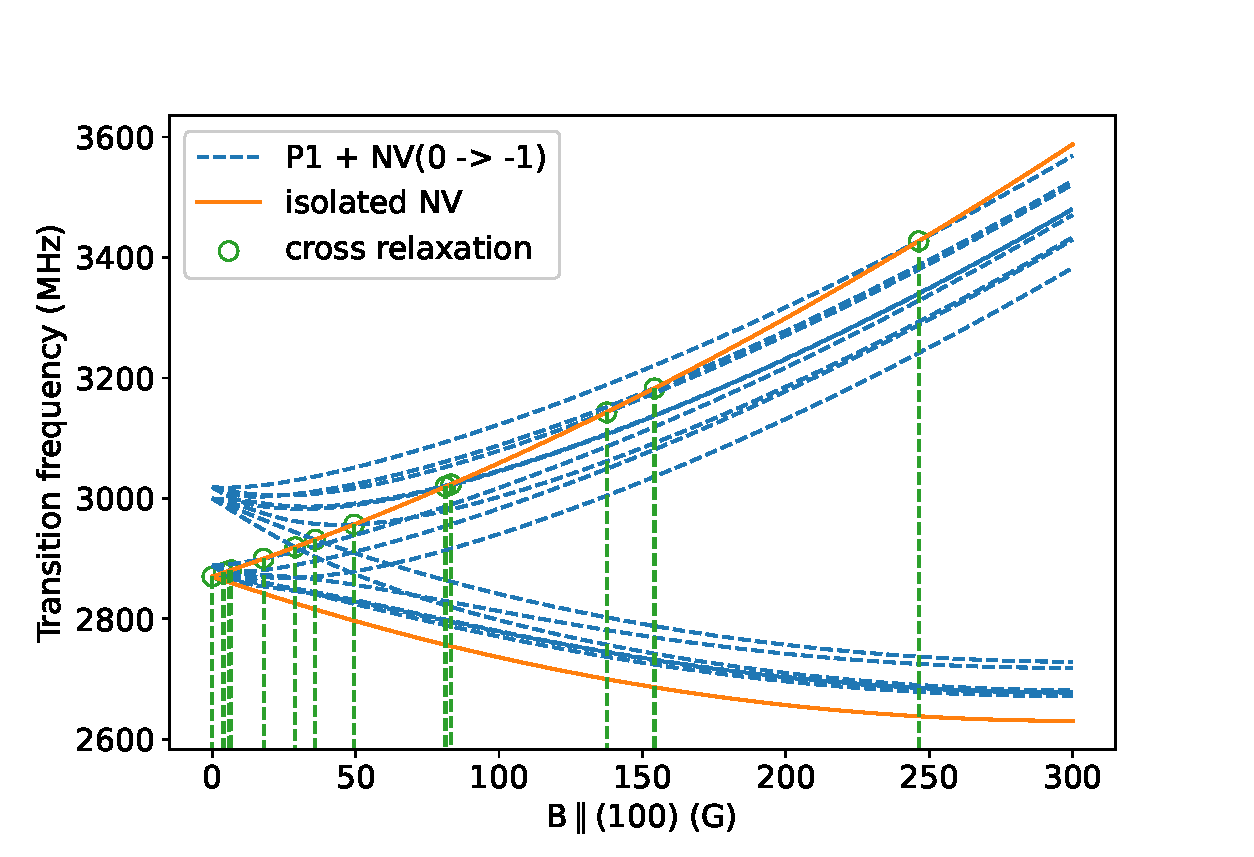
\includegraphics[scale=.6]{Transis_P1}
\caption{Cross-relaxation condition for mutual flip between NV and P1 centers. The orange plain lines correspond to the NV center $\ket{m_s=0} \to \ket{m_s=-1}$ and $\ket{m_s=0} \to \ket{m_s=+1}$ transition frequencies as function of a magnetic field along the [100] crystalline axis, the blue dashed lines correspond to the frequencies of the 15 theoretical transitions of the P1 centers, added to the frequency of the NV $\ket{m_s=0} \to \ket{m_s=-1}$ transition. The green circles correspond to the particular magnetic fields where eq. \ref{eq_P1} is verified, meaning the energy of the P1 transition matches the difference of energy between the two NV transitions.}
\end{figure}
% Bibliography
\bibliographystyle{plain}
\bibliography{Biblio_CVD-CR}

% Full bibliography added automatically for Optics Letters submissions; the following line will simply be ignored if submitting to other journals.
% Note that this extra page will not count against page length





\end{document}
